\usetikzlibrary{shapes.multipart}

\tikzset{block/.style={
        font=\sffamily,
        draw=black,
        thin,
        fill=white!50,
        rectangle split,
        rectangle split horizontal,
        rectangle split parts=#1,
        outer sep=0pt},
        %
        gblock/.style={
            block,
            rectangle split parts=#1,
            fill=green!30}
        }

    
\def\lvld{1.2}                  % Choose level distance
\pgfmathsetmacro\shft{-6*\lvld} % Calculate the yshift for the green tree

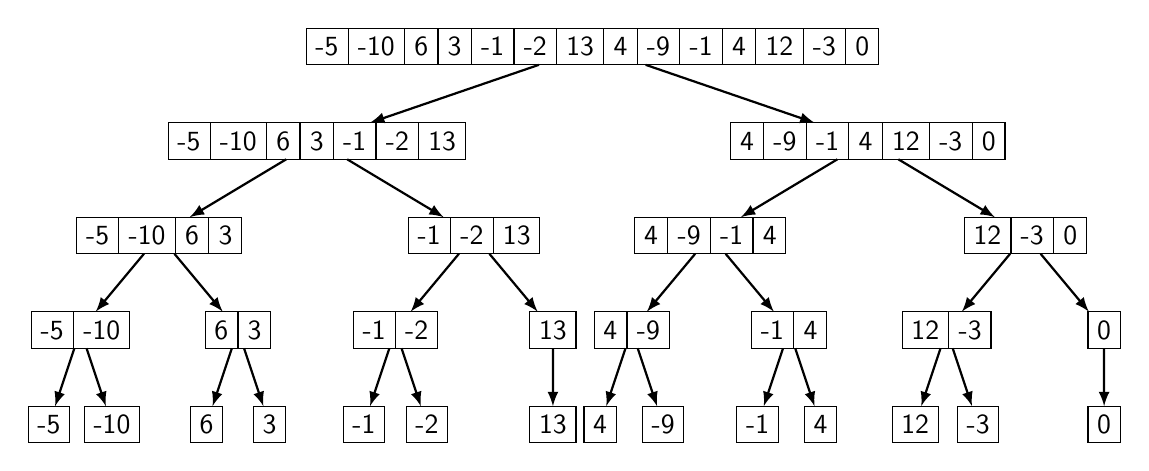
\begin{tikzpicture}[level distance=\lvld cm,
                level 1/.style={sibling distance=7cm},
                level 2/.style={sibling distance=4cm},
                level 3/.style={sibling distance=2cm},
                level 4/.style={sibling distance=0.8cm},
                edgedown/.style={edge from parent/.style={draw=black,thick,-latex}},
                edgeup/.style={edge from parent/.style={draw=green!50!black,thick,latex-}}
                ]


\node[block=14] (A) {-5 \nodepart{two} -10 \nodepart{three} 6 \nodepart{four} 3 \nodepart{five} -1 \nodepart{six} -2 \nodepart{seven} 13 \nodepart{eight} 4 \nodepart{nine} -9 \nodepart{ten} -1 \nodepart{eleven} 4 \nodepart{twelve} 12 \nodepart{thirteen} -3 \nodepart{fourteen} 0}
    [grow=down,edgedown]
    child {node[block=7] (B1) {-5 \nodepart{two} -10 \nodepart{three} 6 \nodepart{four} 3 \nodepart{five} -1 \nodepart{six} -2 \nodepart{seven} 13 }
        child {node[block=4] (C1) {-5 \nodepart{two} -10 \nodepart{three} 6 \nodepart{four} 3 }
            child {node[block=2] (D1) {-5 \nodepart{two} -10}
                child {node[block=1] (E1) {-5}}
                child {node[block=1] (E2) {-10}}
            }
            child {node[block=2] (D2) {6 \nodepart{two} 3}
                child {node[block=1] (E3) {6}}
                child {node[block=1] (E4) {3}}
            }
            }
        child {node[block=3] (C2) {-1 \nodepart{two} -2 \nodepart{three} 13}
            child {node[block=2] (D3) {-1 \nodepart{two} -2} 
                child{node[block=1] (E5) {-1}}
                child{node[block=1] (E6) {-2}}
            }
            child {node[block=1] (D4) {13}
                child{node[block=1] (E7) {13}}
            }
            }
        }
    child {node[block=7] (B2) {4 \nodepart{two} -9 \nodepart{three} -1 \nodepart{four} 4 \nodepart{five} 12 \nodepart{six} -3 \nodepart{seven} 0}
        child {node[block=4] (C3) {4 \nodepart{two} -9 \nodepart{three} -1 \nodepart{four} 4}
            child {node[block=2] (D5) {4 \nodepart{two} -9}
                child {node[block=1] (E8) {4}}
                child {node[block=1] (E9) {-9}}
            }
            child {node[block=2] (D6) {-1 \nodepart{two} 4}
                child {node[block=1] (E10) {-1}}
                child {node[block=1] (E11) {4}}
            }
        }
        child {node[block=3] (C4) {12 \nodepart{two} -3 \nodepart{three} 0}
            child {node[block=2] (D7) {12 \nodepart{two} -3} 
                child{node[block=1] (E12) {12}}
                child{node[block=1] (E13) {-3}}
            }
            child {node[block=1] (D8) {0}
                child{node[block=1] (E14) {0}}
            }
            }
    };
\end{tikzpicture}